In this chapter, we will focus on the detection of so-called cold or hot spots, points characterized by an unusual thermal behavior in the print bed of PBF 3D printers for metallic components. In Section \ref{sec:comelotrovo} I will describe different approaches for defect detection, while in Section \ref{sec:sensoriniiniini} I will describe available sensors used in anomalies detection. Since I want this chapter to be fully-comprehensible to as many readers as possible, whenever I deem it necessary to explain certain aspects of presented methods a little deeper, I will provide a brief introductory overview to elucidate the fundamental aspects in Section \ref{sec:introperritardati}. For a detailed understanding of the research strategy employed to write this state-of-art review, please refer to Appendix \ref{ap:research}. 

\section{Defects Characterization Methods}
\label{sec:comelotrovo}

\section{Sensors for Anomalies Detection}
\label{sec:sensoriniiniini}


\section{Warm Up}
\label{sec:introperritardati}
In this section, I will explain some fundamental concepts that are essential for fully understanding the subsequent sections. If the reader is already familiar with these concepts, they can comfortably skip this section and proceed further. 

% Machine learning>>>
\subsection{Machine Learning}
\label{subsec:ml}
In recent years, the volume of data and the speed at which it becomes available have increased exponentially. Thus, there is the need for new tools, we can lever in order to find valuable and actionable insights from these huge amount of data. The set of activities involved in the analysis of these large databases, usually with the purpose of extracting useful knowledge to support decision making, has been referred as \emph{machine learning}\cite{vercellis_business_2009}. Machine Learning (ML) is a subset of artificial intelligence that involves the development of algorithms that enable computers to learn from and to find patterns in a large amount of data. Rather than being explicitly programmed to perform a task, a machine learning system uses inference to make predictions or decisions based on input data. Formally, “A computer program is said to learn from experience E with respect to some class of task $T$ and a performance measure $P$, if its performance at tasks in $T$, as measured by $P$, improves because of experience $E$” \cite{zaki_data_2020, pierluca_lanzi_data_2021}. Suppose we have the experience $E$, a set of observations of a specific phenomenon, encoded as a dataset
\begin{equation}
    \label{eq:dataset}
    D=\{\mathbf{X}_1, \dots, \mathbf{X}_N\} 
\end{equation}
where $\mathbf{x}_i\in \mathbb{R}^p$ is a $p$ dimensional vector, containing the realization of the $p$ features of the dataset. We have three possible scenarios:
\begin{itemize}
    \item \textbf{Supervised learning:} given the desired outputs $\textbf{t}_1, \textbf{t}_2, \dots, \textbf{t}_N$, also known as labels, the algorithm learns how to produce the correct output given a new set of input;
    \item \textbf{Unsupervised learning:} given $D$, the algorithm is used to exploit regularities, usually used as input for supervised learning algorithm, for explaining the observations or for prediction.
    \item \textbf{Reinforcement learning:} the algorithm producing actions $a_1, a_2, \dots, a_H$ which affect the environment, and receiving rewards $r_1, r_2, \dots, r_H$, learn how to act in order to maximize rewards in the long term.
\end{itemize}
To further highlight the difference between supervised and unsupervised learning, it's important to note that unsupervised learning is also defined as "learning without a teacher" in \citeauthor{tibshirani_elements_2008} (2008). So, the main difference between supervised and unsupervised learning is the input data: in former case, data is labeled a priori, while in the latter case is not. 
% <<< end of Machine learning

% Clustering algorithms >>>
\subsection{Clustering Algorithms}
\label{sec:clustering}
Clustering is an unsupervised learning technique. The aim of all \emph{clustering algorithms} is to organize a collection of entities $D$ into subsets or "clusters" wherein elements within a cluster are as similar as possible, whereas data in different clusters are as dissimilar as possible. So, the goal of clustering is to minimize the within-clusters variance while maximizing the between-clusters variance. But how do we define if two observations in $D$ are similar? We have to rely on the concept of distance between the two observations. There are several different definitions of distances. In general, given a space $\mathbb{R}^p$ and a set of points on this space, a distance measure $d\left(\mathbf{X}_1,\mathbf{X}_2\right)$ is a function mapping two points $\mathbf{X}_1\in\mathbb{R}^p$ and $\mathbf{X}_2\in\mathbb{R}^p$ to a real number, and satisfies these axioms:
\begin{enumerate}
    \item $d\left(\mathbf{X}_1,\mathbf{X}_2\right) \geq 0$
    \item $d\left(\mathbf{X}_1,\mathbf{X}_2\right) = d\left(\mathbf{X}_2,\mathbf{X}_1\right)$
    \item $d\left(\mathbf{X}_1,\mathbf{X}_2\right)=0 \Leftrightarrow \mathbf{X}_1 = \mathbf{X}_2$
    \item $d\left(\mathbf{X}_1,\mathbf{X}_2\right) \leq d\left(\mathbf{X}_1,\mathbf{X}_3\right) + d\left(\mathbf{X}_1,\mathbf{X}_3\right)$
\end{enumerate}
where $\mathbf{X}_3 \in \mathbb{R}^p$ is a third point in the space. Recalling that $\mathbf{X}_1=\left(x_{11}, x_{12}, \dots, x_{1p} \right)$ and $\mathbf{X}_1=\left(x_{21}, x_{22}, \dots, x_{2p} \right)$, most used distance measure:
\begin{itemize}
    \item Euclidean distance
\begin{equation}
    \label{eq:euclidean}
    d\left(\mathbf{X}_1,\mathbf{X}_2\right) = \sqrt{\sum_{i=1}^p\left(x_i-y_i \right)}
\end{equation}
\item Manhattan distance
\begin{equation}
    \label{eq:mandistance}
    d\left(\mathbf{X}_1,\mathbf{X}_2\right) = \sum_{i=1}^p\left|x_i-y_i \right|
\end{equation}

\item Mahalanobis distance
\begin{equation}
    \label{eq:mahadistance}
    d(\mathbf{X}_1, \mathbf{X}_2) = \sqrt{(\mathbf{X}_1 - \mathbf{X}_2)^\mathrm{T} \Sigma^{-1} (\mathbf{X}_1 - \mathbf{X}_2)}
\end{equation}
where $\Sigma^{-1}$ it's the inverted covariance matrix
\item Jaccard distance, used in the case of cathegorical features, once they have been encoded using one-hot encoding
\begin{equation}
    \label{eq:jaccard}
    d\left(\mathbf{X}_1, \mathbf{X}_2\right) = 1 - J\left(\mathbf{X}_1, \mathbf{X}_2\right)
\end{equation}
where 
\begin{equation}
J\left(\mathbf{X}_1, \mathbf{X}_2\right) = \frac{\left|\mathbf{X}_1 \cap \mathbf{X}_2\right|}{\left|\mathbf{X}_1 \cup \mathbf{X}_2\right|}    
\end{equation}
\end{itemize}
There are several different clustering algorithms that can be divided into two main groups, as in \citeauthor{james_introduction_2021} (2021): K-Means clustering and hierarchical clustering. In \emph{K-Means clustering}, we try to divide observation into a pre-specified number of clusters. On the other hand, in \emph{hierarchical clustering}, we do not specify the number of clusters in advance, but we rely on the dendrogram, a tree-like visual representation of the observations, that allows us to visualize all the clustering steps. Then, we can then "cut" the dendrogram in order to select the most appropriate number of cluster to us. In Fig. \ref{fig:clustiteration} there is an example of simulated data in the plane clustered into 3 clusters using the K-Means algorithm (that will be discussed later).

\subsubsection{K-Means Clustering Algorithm}
\label{sss:kmeans}
Since we will use K-Means, in Section \ref{sec:bvc} or in Appendix \ref{ap:Python}, we will delve deeper into it in a dedicated section. Let $C_1,\dots,C_k$ denotes the sets containing all the indices of the observation in respective the respective cluster. K-Means clustering is a very simple clustering algorithm we can use for complete partitioning a data collection of observations $\mathbf{x}=\left(X_1, \dots, X_p \right)$, described by $p$ features, into $K$ distinct, non-overlapping clusters. This means that:
\begin{enumerate}
    \item $C_1 \cup C_2 \cup \dots \cup C_K=\{1,\dots,n\}$. So, each observation belongs to at least one of the $K$ clusters.
    \item $C_k\cap C_{k'}=0$ for all $k\neq k'$. In other words, there is no observation belonging to more than one cluster.
\end{enumerate}
Thus, each observation will be assigned to one cluster and one cluster only. Moreover, for every cluster $C_i$, there is a representative point that summarize the cluster. That's the centroid $\bm{\mu}_i$
\begin{equation}
    \label{eq:centroid}
    \boldsymbol{\mu}_i=\frac{1}{\left|C_i\right|} \sum_{x_j \in C_i} \mathbf{x}_j
\end{equation}
K-means begins by randomly placing $\bm{\mu}_i \in \mathbb{R}^p$ for $i=1,\dots,K$ points as initial cluster centroids. This is usually achieved by generating a random value within the bounds of each dimension. 
\begin{figure}[H]
    \centering
    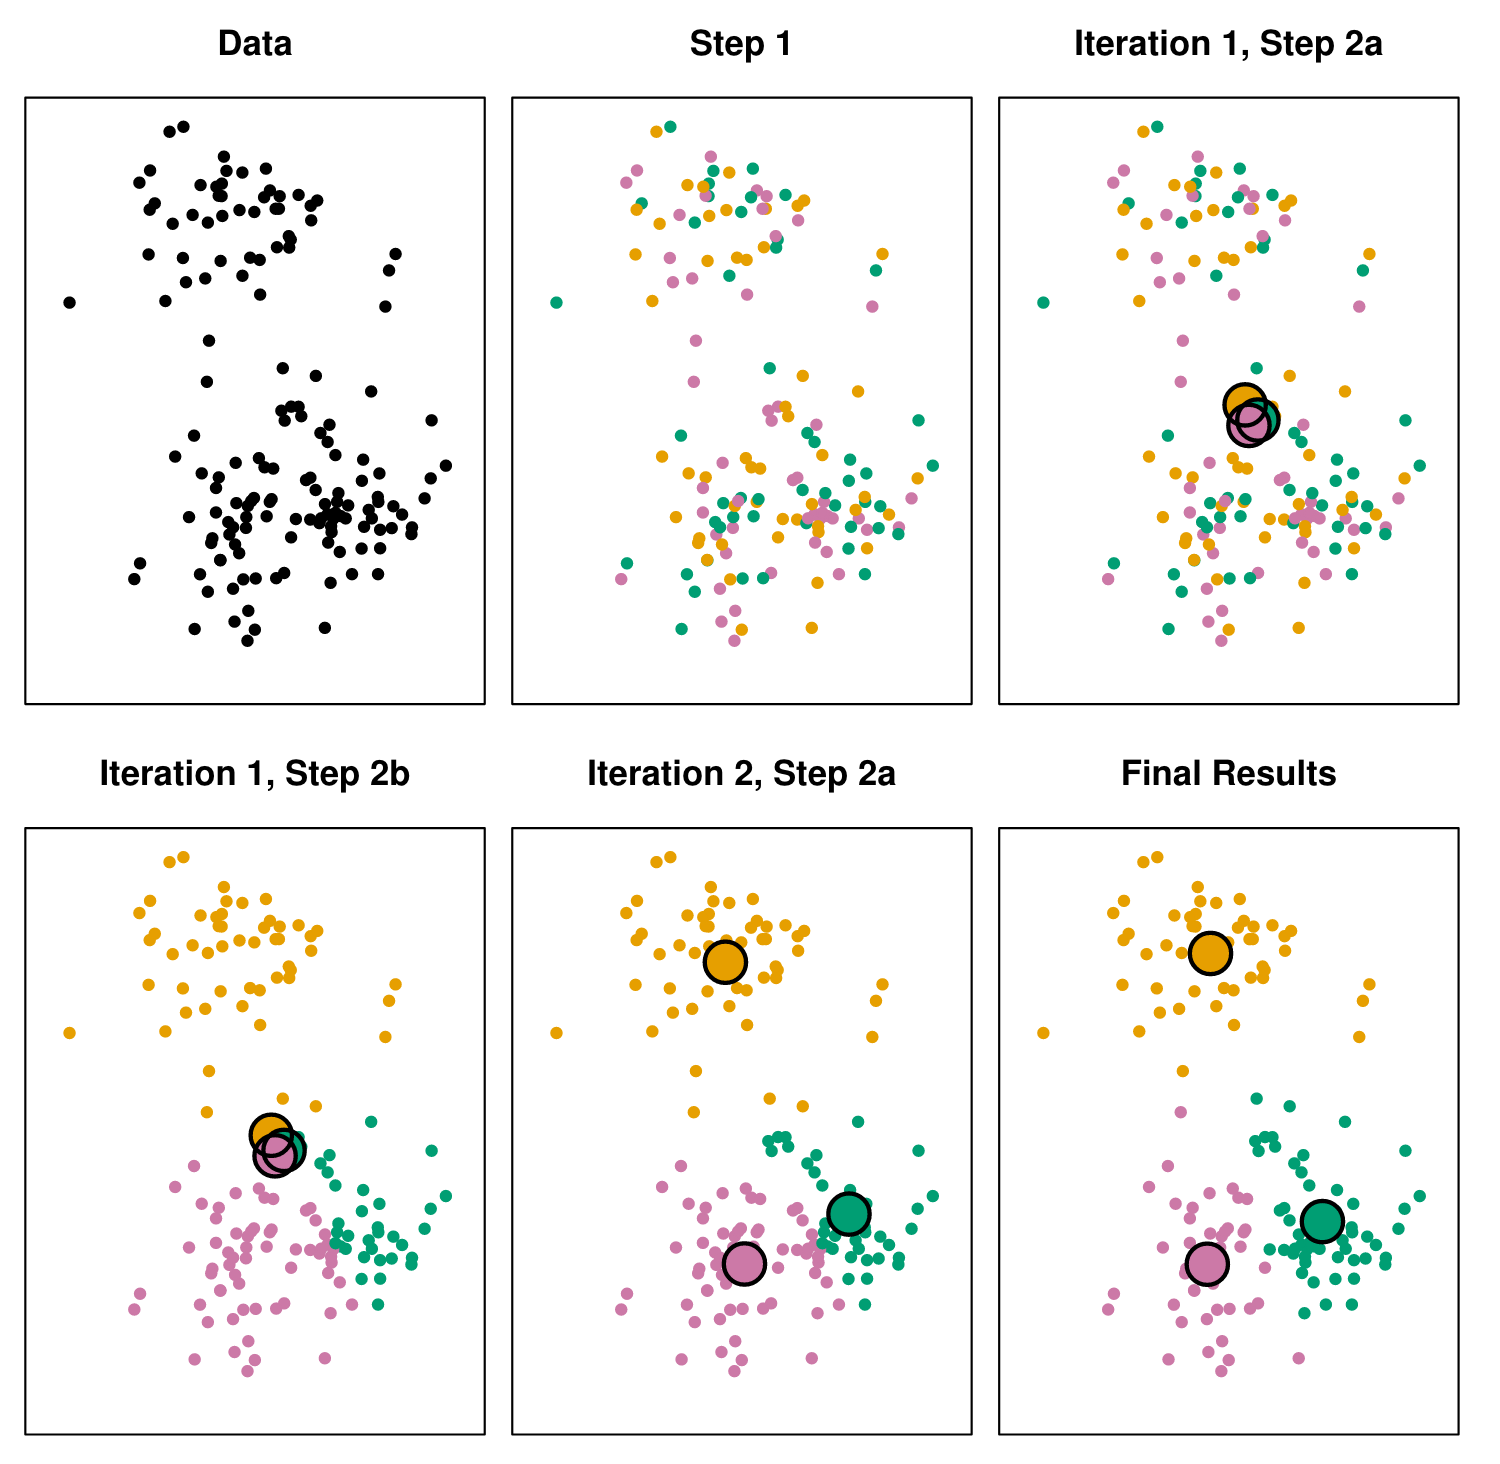
\includegraphics[width=0.6\textwidth]{Images/clustiteration.png}
    \caption[K-Means clustering iterations.]{The progress of the K-means algorithm with $K=3$ \cite{james_introduction_2021}.}
    \label{fig:clustiteration}
\end{figure}
The K-means algorithm progresses through iterative cycles, involving two primary actions: (1) assigning data points to clusters, and (2) updating centroids. Given the $K$ centroids, the assignment phase allocates each data point to its nearest centroid, resulting in distinct clusters, where each cluster $C_i$ consists of points nearer to its centroid $\bm{\mu}_i$ than to any other centroid. Then, in the centroid modification phase, each cluster's centroid is recalculated based on its (updated) member data points. This iterative process of assignment and updating continues until the centroids stabilize or reach a local minimum. In practical terms, K-means can be considered as having reached convergence when there's no shift in centroid positions between consecutive iterations. We can adjust the tolerance parameter $\epsilon \geq 0$ for an early termination of the algorithm, or let the algorithm converge to the local optimum until observations don't change cluster anymore. In algorithm \ref{alg:kmeans} there is the pseudo-code of K-Means clustering algorithm.
\begin{algorithm}[H]
\small
    \caption{K-Means Clustering}
    \label{alg:kmeans}
    \begin{algorithmic}[1]
    \STATE {$t=0$}
    \STATE {Randomly initialize $K$ centroids: $\bm{\mu}_1^t, \bm{\mu}_2^t, \dots, \bm{\mu_k^t} \in \mathbb{R}^p$}
    \REPEAT
    \STATE {$t \leftarrow t + 1$}
    \STATE {$C_i \leftarrow \empty$ for all $i=1,\dots,K$}
    \STATE {//Cluster assignment step}
    \FORALL{$\mathbf{X}_j\in D$}
    \STATE {$i^* \leftarrow \arg \min _i\left\{\left\|\mathbf{X}_j-\boldsymbol{\mu}_i^{t-1}\right\|^2\right\}$}
    \STATE {$C_{i^*} \leftarrow C_{i^*} \cup\left\{\mathbf{x}_j\right\} / / \text { Assign } \mathbf{x}_j \text { to closest centroid }$}
    \ENDFOR
    \STATE {//Centroid update Step}
    \FORALL{$i=1,\dots,K$}
    \STATE{$\boldsymbol{\mu}_i^t \leftarrow \frac{1}{\left|C_i\right|} \sum_{\mathbf{x}_j \in C_i} \mathbf{x}_j$}
    \ENDFOR
    \UNTIL{$\sum_{i=1}^k\left\|\boldsymbol{\mu}_i^t-\boldsymbol{\mu}_i^{t-1}\right\|^2 \leq \epsilon$}
    \end{algorithmic}
\end{algorithm} 
In bagging clustering, since the initial guess of the centroids can lead to different labeling of the same observation, K-means algorithm is typical run several times. Then, final label will be defined by majority voting across the different intermediate clusterization.
% <<< End of Unsupervised classification

\subsection{Artificial Neural Network and Deep Learnig}
\label{subsec:deepl}
It was 1956 when a team of professors and an expert from IBM Corporation, after spending two months discussing artificial intelligence at Dartmouth University, began to think about the possibility of creating virtual neural networks. These networks would learn and enhance the purpose for which they were designed through a self-improvement process, and they could be founded on the mathematical model of the human brain \cite{mccarthy_proposal_1955}. Indeed, the model of the human brain is especially well-suited for translation into the field of computer science. The human brain possesses an astonishingly vast number of computing units, known as neurons. There are approximately \num{10e11} neurons in the human brain, and each of them is forming about 7,000 synaptic connections with other neurons, amounting to nearly \num{5e14} total synapses in an adult. Moreover, the computational model of the brain is distributed among simple nonlinear units, it is redundant and so fault-tolerant, and it is capable of performing calculations in parallel \cite{matteo_matteucci_perceptrons_2021}. The mathematical virtual model of a neuron is called a perceptron, which is the unitary computational units of artificial neural networks (ANN). Just like in human neurons, the perceptron has dendrites that "collect" the charge from synapses, and once a certain threshold is exceeded, the accumulated charge is released and sent to other perceptrons. The portion of the schema in Fig. \ref{fig:perceptron} enclosed in the dashed line, is called activation function and is responsible for releasing perceptron's accumulated charge. There are various activation functions, with some of the most common ones can be seen in Fig. \ref{fig:actfunc}.
\begin{figure}
    \centering
    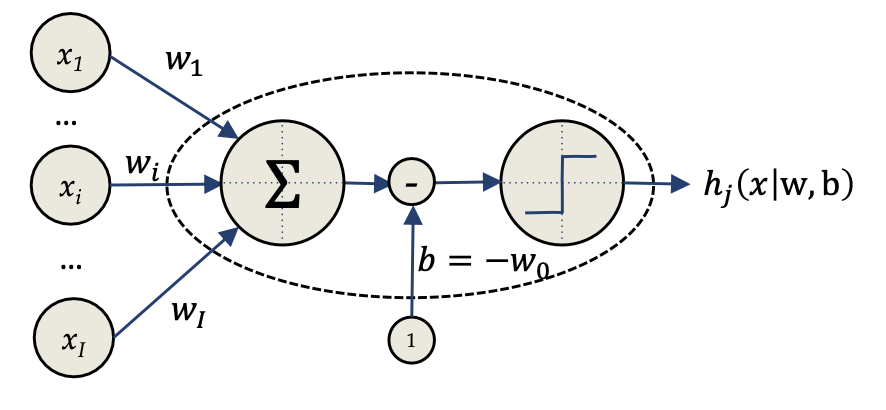
\includegraphics[width=0.6\textwidth]{Images/neurone.png}
    \caption[Perceptron schema]{Perceptron schema \cite{matteo_matteucci_perceptrons_2021}.}
    \label{fig:perceptron}
\end{figure}
Perceptrons can be combined together to form networks with a layered architecture. Indeed, every neural network will have an input layer, an output layer, and a varying number of intermediate layers, known as hidden layers. Deep learning is a subfield of artificial intelligence (AI) and machine learning that involves training artificial neural networks on vast amounts of data to perform classification or regression tasks. ANN are capable to learn from experience $E$ and undestand complex patterns in data. Deep feedforward networks, also often called feedforward neural networks, or multilayer perceptrons (MLPs), are used to approximate some function $f^*$. Let's take as example a classifier. Given an unknown function $\Lambda_0:E \rightarrow \{1,\dots,L\}$ where $\{1,\dots,L\}$ are the classes, the $f^*$ is the best approximation of the function $\Lambda_0$, defining a mapping $\mathbf{y}=f^*\left(\mathbf{x}, \bm{\theta} \right)$. Value of parameters $\bm{\theta}$ are learn from $E$, resulting in the best function approximation. These models are called feedforward because information flows through the function being evaluated from $\mathbf{x}$, through the intermediate computations used to define $f^*$, and finally to the output $\mathbf{y}$. To understand how neural networks learn from experience $E$ using the chain rule and the back-propagation mechanism, readers are referred to \citeauthor{goodfellow_deep_2016}.
\begin{figure}
    \centering
    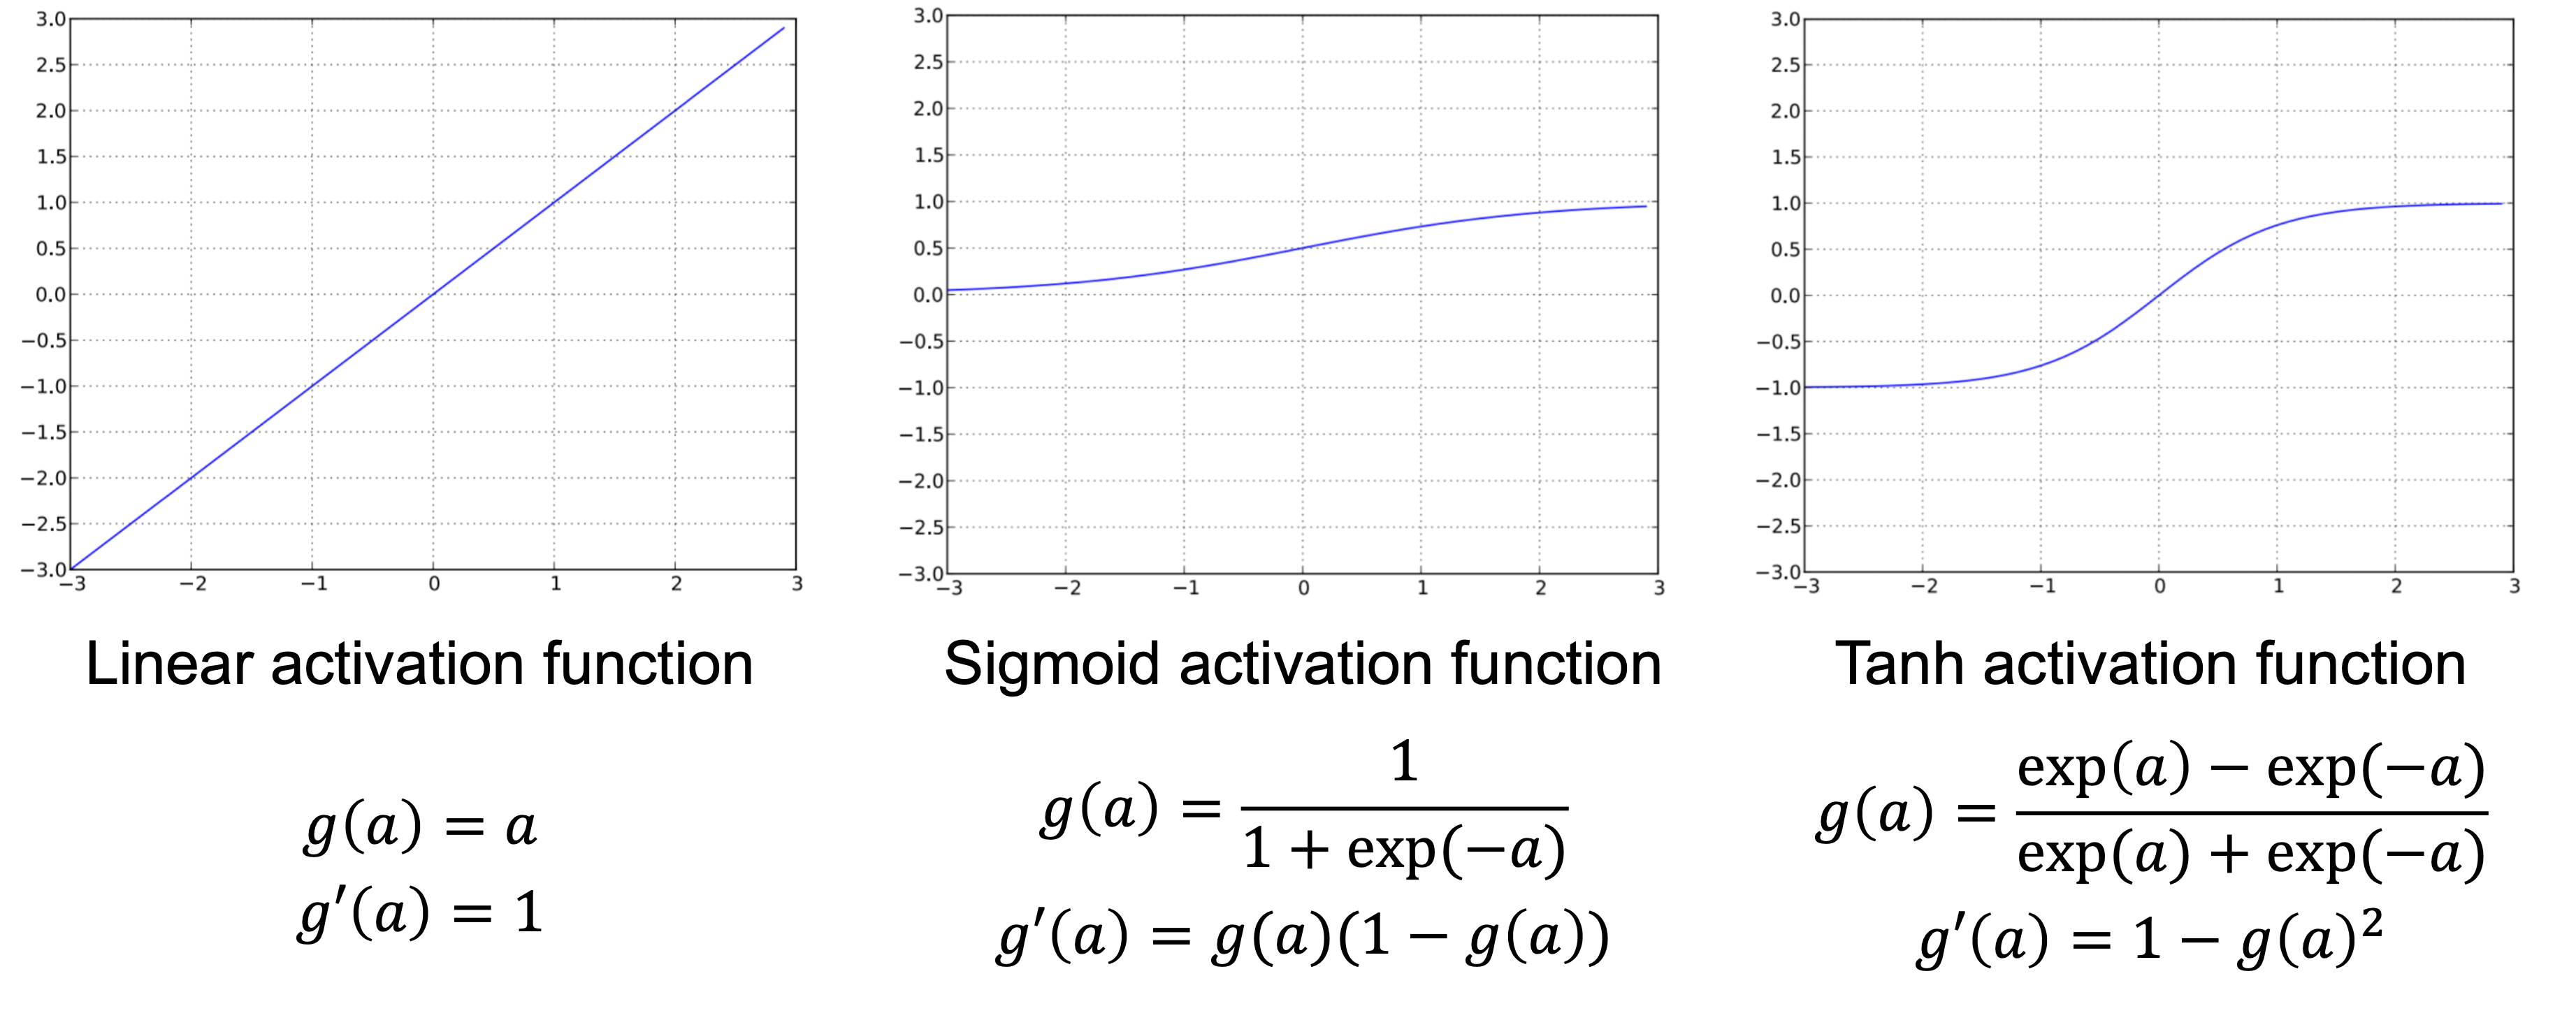
\includegraphics[width=0.8\textwidth]{Images/activationfunction.png}
    \caption[Activation functions.]{Some examples of activation functions with relatives analytical forms \cite{matteo_matteucci_perceptrons_2021}.}
    \label{fig:actfunc}
\end{figure}
Let's examine some examples of how networks can be used to address classic machine learning problems such as regression and classification. Best practice is to use tanh or sigmoid as the activation function for the hidden layers. Indeed, the difference is the activation function of the output layer: 
\begin{itemize}
    \item \textbf{Regression:} since the output of a regression problem spans all $\mathbb{R}$, the activation function of the output layer will be a linear activation function;
    \item \textbf{Binary Classification:} in binary classification, the output domain is $\Omega=\{0, 1\}$, thus the necessary activation function for the output layer is the sigmoid activation function (it can be interpreted as class posterior probability);
    \item \textbf{Multi-class Classification:} when dealing with multiple classes ($K$) use as many neuron as classes and each output neuron will use softmax unit. The unique feature of this activation function is that the sum of the outputs from the $K$ output neurons is equal to 1. Thus, the $k$-th output can be viewed as the probability that the input belongs to $k$-th class.
\end{itemize}
Another typical application of neural networks is as classification algorithms for images in computer vision. However, images cannot be used directly as input. We need some intermediate steps to extract useful information and reduce the problem's dimensionality \cite{giacomo_boracchi_convolutional_2021}. The feature array for the input layer will have a dimension of $d\ll r_1 \times c_1$ where $r_1$ and $c_1$ are the rows and the columns of the matrix representation of the image. Recall that an image can be represented as a three-dimensional matrix, with the first two dimensions indexing the pixels and the third identifying the pixel's color based on the color profile used. Take, for instance, the image in figure \ref{fig:cazzle}. The image has a width of 472 pixels, a height of 376 pixels, and uses an RGB color profile. This means that three values are needed to uniquely identify the color of each pixel: the first for red, the second for green, and the third for blue. This means that we would require 472 $\times$ 376 $\times$ 3 input neurons, one for each value of each color of each pixel of the image (more than 500,000 neurons). Feature extraction algorithms can be categorized as hand-crafted or data-driven features. With the former, we can leverage prior knowledge of the phenomenon, and features are interpretable, allowing us to exploit them even with a limited amount of data. However, this approach demands significantly more time and design/programming efforts and is not as general and "portable". On the other hand, data-driven feature extraction algorithms are less interpretable but offer a more robust mathematical foundation as input for classification algorithm. Convolutional Neural Networks (CNNs) are types of neural networks that can be used for data-driven feature extraction. Given the matrix representation of the image discussed earlier, while in ANN we referred to layers, in CNNs we will discuss volumes, and as the depth increases the height and width of the volume decreases. CNNs enable us to perform some fundamental operations essential for accurate feature extraction.
\begin{figure}
    \centering
    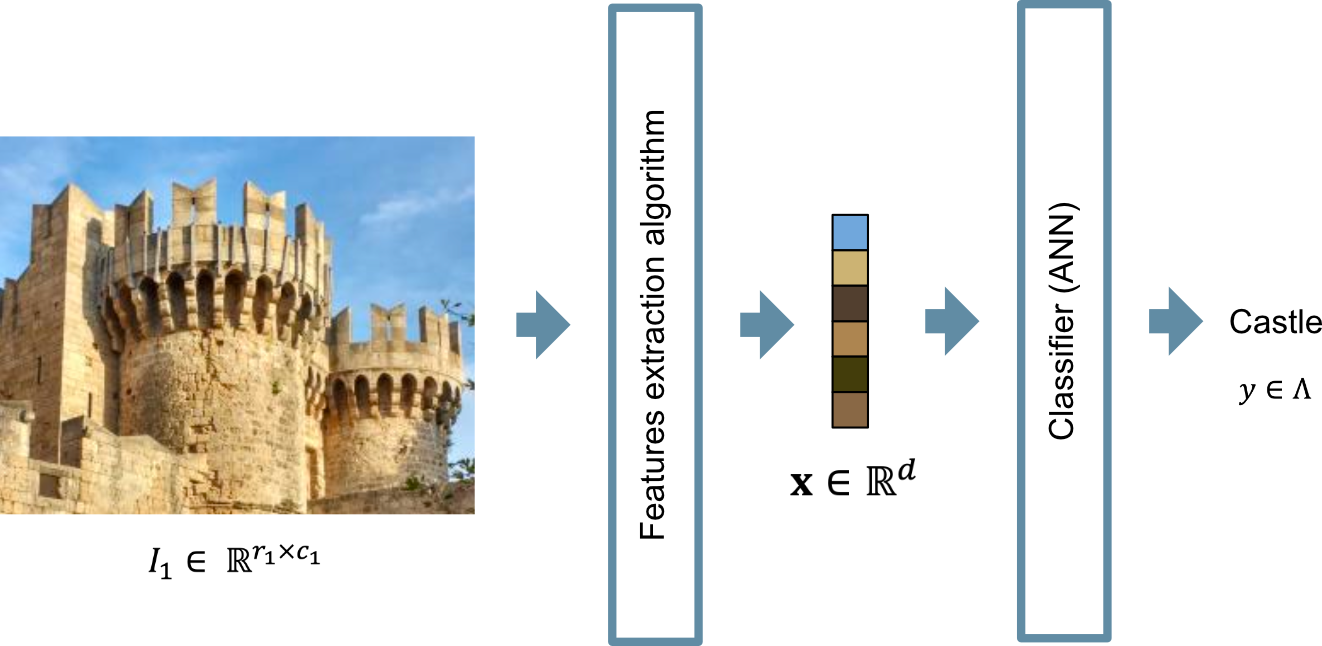
\includegraphics[width=0.7\textwidth]{Images/featureextraction.png}
    \caption[Feature extraction perspective.]{Feature extraction perspective. Adapted from \cite{giacomo_boracchi_convolutional_2021}.}
    \label{fig:cazzle}
\end{figure}

\paragraph{Convolution}
\paragraph{Poolig layers}